\documentclass{beamer}
\usepackage{graphicx}
\usetheme{AnnArbor}

\begin{document}
\section{Workshop on Qt}
\title{Programming with the Qt Framework}
\author{Saurabh Sood}

\begin{frame}
\titlepage
\end{frame}

\begin{frame}{Table Of Contents}
\tableofcontents
\end{frame}

\section{A bit of introduction}
\begin{frame}{What is a framework?}
\pause
\begin{itemize}
\item A collection of tools and libraries to make certain tasks easier? \pause
\begin{itemize}
\item Eg: A Dynamic Array, Hashtables etc (Collections)
\item Generic Algorithms to achieve a certain task
\end{itemize}
\end{itemize}
\end{frame}

\section{About Qt}
\begin{frame}{What is Qt?}\pause
\begin{itemize}
\item Pronounced as 'Cute' ;) \pause
\item It is a \textit{cross platform}, development framework
\item Original Language is C++ with bindings in many languages (Ruby, Python etc) \pause
\end{itemize}
\end{frame}

\begin{frame}{Supported Platforms}
\pause
\begin{itemize}
\item *nix platforms
\item Windows
\item Android (through Necessitas)
\end{itemize}
\end{frame}

\section{Features}
\begin{frame}{Some features of Qt}
\begin{itemize}
\pause
\item Modular Design
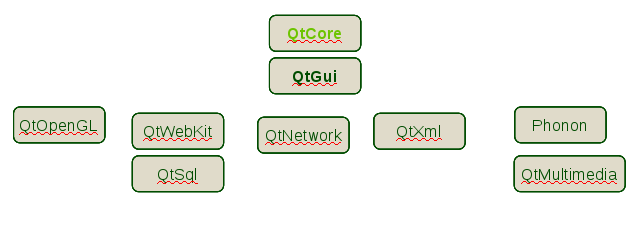
\includegraphics[width=10cm]{qt-mod.png}
\end{itemize}
\end{frame}

\begin{frame}{Macros and Introspection}
\pause
\begin{itemize}
\item Qt extends with \textit{macros} and \textit{introspection}
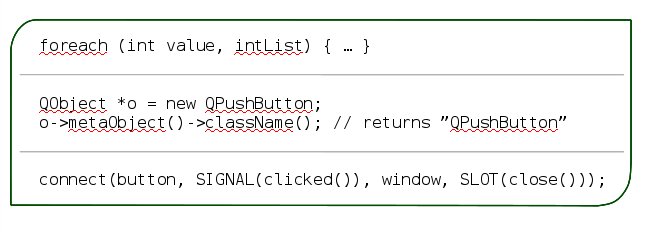
\includegraphics[width=10cm]{macros.png}
\end{itemize}
\end{frame}

\begin{frame}{Meta Data and MOC}
\begin{itemize}
\item Every \textit{QObject} has a \textit{meta object}
\item The meta object knows about certain properties related to the class such as \textit{class name}, \textit{inheritance}, \textit{signals and slots} etc
\item The moc looks for macros like \textit{signals}, \textit{slots} etc
\item Introspection refers to the class knowing about its own members at runtime (eg: class name, inheritance structure etc)
\end{itemize}
\end{frame}

\begin{frame}{Applications using it...}
\pause
\begin{itemize}
\item KDE (The whole desktop environment along with the application suite)
\item VLC Media Player
\item Adobe Photoshop
\end{itemize}
\end{frame}

\section{Lets Dig in...}
\begin{frame}{Appease the Programming Gods...}
Hello World!!!
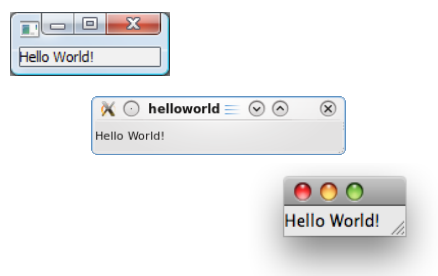
\includegraphics[width=10cm]{helloworld.png}
\end{frame}

\begin{frame}{Appease the Programming Gods...}
Hello World!!!
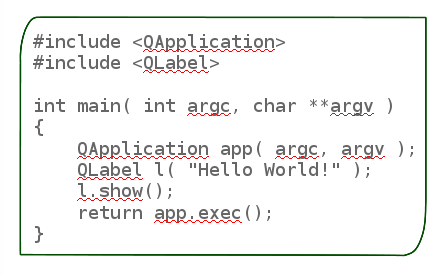
\includegraphics[width=10cm]{helloworld1.png}
\end{frame}

\begin{frame}{A Section by section disection of the code...}
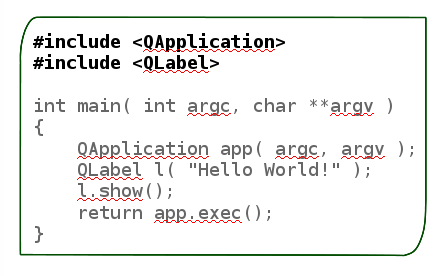
\includegraphics[width=10cm]{helloworld2.png}
\end{frame}

\begin{frame}{A Section by section disection of the code...}
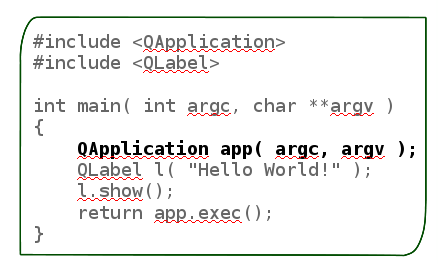
\includegraphics[width=10cm]{helloworld3.png}
\end{frame}

\begin{frame}{A Section by section disection of the code...}
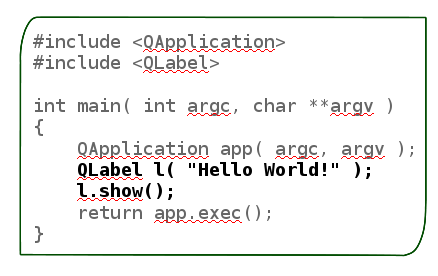
\includegraphics[width=10cm]{helloworld4.png}
\end{frame}


\begin{frame}{A Section by section disection of the code...}
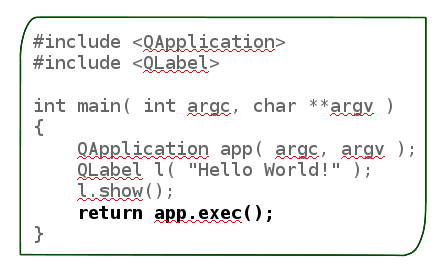
\includegraphics[width=10cm]{helloworld5.png}
\end{frame}

\section{Qt's event handling mechanism}
\begin{frame}{Signals and Slots}
\begin{itemize}
\pause
\item Qt's \textit{callback} mechanism \pause
\item Dynamically ties together events and state changes with reactions \pause
\item What makes Qt tick!!! ;)
\end{itemize}
\end{frame}

\begin{frame}{Slots}
\begin{itemize}
\item \textit{Callback} methods \pause
\item Defined as normal methods but with the slot macro \pause
\item A number of signals can be connected to the same slot \pause
\item Can be called as an ordinary method
\end{itemize}
\end{frame}

\begin{frame}{Signals}
\begin{itemize}
\item Events, State Changes \pause
\item Return void \pause
\item Must not be implemented. The \textit{moc} provides an implementation \pause
\item Can be emitted using the \textit{emit} keyword
\end{itemize}
\end{frame}

\begin{frame}{Making the connection}
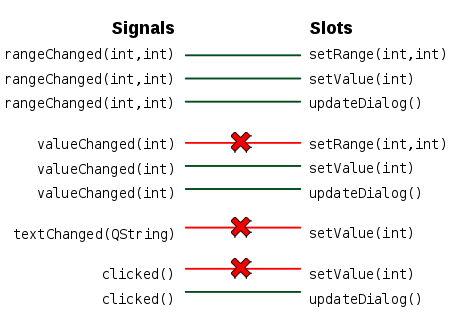
\includegraphics[width=10cm]{sigslots.png}
\end{frame}

\begin{frame}{Making the connection}
Connection done through the \textit{connect} method
\\ \textit{connect(src, SIGNAL(sig()), dest, SLOT(doSomething());}
\end{frame}

\section{Lets Code...}
\begin{frame}{Getting our hands dirty...}
Looking at some code...
\end{frame}

\section{Some Helpful Links}
\begin{frame}{Where I can learn some more...}
\begin{itemize}
\item Qt project site - http://qt-project.org/doc
\item Advanced Qt Programming - http://www.qtrac.eu/aqpbook.html
\end{itemize}
\end{frame}


\section{Questions???}
\begin{frame}{Questions???}
\pause
\end{frame}

\end{document} 
